\documentclass[letterpaper,10pt]{article}

\usepackage{titling}
\usepackage{listings}
\usepackage{url}
\usepackage{setspace}
\usepackage{subfig}
\usepackage{sectsty}
\usepackage{pdfpages}
\usepackage{colortbl}
\usepackage{multirow}
\usepackage{multicol}
\usepackage{relsize}
\usepackage{amsmath}
\usepackage{fancyvrb}
\usepackage[yyyymmdd]{datetime}
\usepackage{amsmath,amssymb,amsthm,graphicx,xspace}
\usepackage[titlenotnumbered,noend,noline]{algorithm2e}
\usepackage[compact]{titlesec}
\usepackage{XCharter}
\usepackage[T1]{fontenc}
\usepackage{tikz}
\usetikzlibrary{arrows,automata,shapes,trees,matrix,chains,scopes,positioning,calc}
\tikzstyle{block} = [rectangle, draw, fill=blue!20, 
    text width=2.5em, text centered, rounded corners, minimum height=2em]
\tikzstyle{bw} = [rectangle, draw, fill=blue!20, 
    text width=4em, text centered, rounded corners, minimum height=2em]

\definecolor{namerow}{cmyk}{.40,.40,.40,.40}
\definecolor{namecol}{cmyk}{.40,.40,.40,.40}
\renewcommand{\dateseparator}{-}


\let\LaTeXtitle\title
\renewcommand{\title}[1]{\LaTeXtitle{\textsf{#1}}}


\newcommand{\handout}[5]{
  \noindent
  \begin{center}
  \framebox{
    \vbox{
      \hbox to 5.78in { {\bf ECE252: Systems Programming and Concurrency } \hfill #2 }
      \vspace{4mm}
      \hbox to 5.78in { {\Large \hfill #4  \hfill} }
      \vspace{2mm}
      \hbox to 5.78in { {\em #3 \hfill \today } }
    }
  }
  \end{center}
  \vspace*{4mm}
}

\newcommand{\lecture}[3]{\handout{#1}{#2}{#3}{Lecture #1}}{
\newcommand{\tuple}[1]{\ensuremath{\left\langle #1 \right\rangle}\xspace}

\addtolength{\oddsidemargin}{-1.000in}
\addtolength{\evensidemargin}{-0.500in}
\addtolength{\textwidth}{2.0in}
\addtolength{\topmargin}{-1.000in}
\addtolength{\textheight}{1.75in}
\addtolength{\parskip}{\baselineskip}
\setlength{\parindent}{0in}
\renewcommand{\baselinestretch}{1.5}
\newcommand{\term}{Spring 2019}

\singlespace


\begin{document}

\lecture{ 5 --- Process State }{\term}{Jeff Zarnett}

\section*{Process State}

The OS is responsible for determining which programs run when and how to allocate resources. The current state of the process is therefore important information. To maintain the state of the process the PCB has a variable, but we will think about this as a finite state machine (FSM): there are a limited number of states and defined transitions between them. 

\subsection*{The Two-State Model}

Let us begin with the simplest possible model: the two state model. At any time, either a process is executing, or it is not. Thus we have the two states: 

\begin{enumerate}
	\item \textbf{Running:} Actively executing right now.
	\item \textbf{Not Running:} Not currently executing.
\end{enumerate}

When a new process is created, the PCB is allocated and the state of the process is Not Running. Whatever process is currently running, and when the process that currently running is finished or a process switch takes place, the running program's state is changed to Not Running, a new process is selected to run (according to scheduling), and it is put in the Running state while it executes.

\begin{center}
\includegraphics[width=0.65\textwidth]{images/2-state-model.png}\\
State diagram for the two state model.
\end{center}

There are the following transitions in the diagram:
\begin{itemize}
	\item \textbf{Create:} The process is created and enters the Not Running state.
	\item \textbf{Dispatch:} A process that is not currently running begins executing and moves to the Running state.
	\item \textbf{Suspend:} A running program pauses execution, for whatever reason, and moves to the Not Running state.
	\item \textbf{Exit:} A running program finishes, reaching the \texttt{exit}, and can be removed from the list of processes.
\end{itemize}


The two-state model, is, however, inadequate. It assumes that every process is constantly ready to run, which is not a safe assumption. We will need a way to indicate that a process is not ready to run, and thus a third state.

\subsection*{The Three-State Model}

A program that requests a resource like I/O or memory may not get it right away. This is not to say the program will never get it, just that it does not have it right now. Sometimes the program needs user input, and as far as the computer is concerned, the user moves at glacial speed. In any case, the program wants to continue but cannot until it gets what it is waiting for.  If the scheduler picks a process that is waiting for user input, nothing will be happening while the program is waiting for input, so the CPU's time would be wasted. Thus, we should be able to mark a process as ``not ready to proceed'', and we then go to a three-state model:

\begin{enumerate}
 \item \textbf{Running:} Actively executing right now.
 \item \textbf{Ready:} Not running, but ready to execute if selected by the scheduler.
 \item \textbf{Blocked:} Not running, and not able to run until some event happens.
\end{enumerate}

This new state, Blocked, indicates that the program is not ready to run for lack of a resource. It may also be called the Waiting state. The scheduler will not choose a Blocked process to run, even if the CPU has nothing else to do. Suppose process $P_{n}$ is waiting for user input. When the user input is received, an interrupt is generated and the interrupt handler runs. The handler takes the input from the I/O device (keyboard), delivers it to $P_{n}$, then moves the state of $P_{n}$ to Ready.

\begin{center}
\includegraphics[width=0.65\textwidth]{images/3-state-model.png}\\
State diagram for the three-state model.
\end{center}

There are six transitions in the diagram:
\begin{itemize}
	\item \textbf{Create:} The process is created and enters the Ready state.
	\item \textbf{Dispatch:} A process that is not currently running begins executing and moves to the Running state.
	\item \textbf{Suspend:} A running program pauses execution, but can still run if allowed, and moves to the Ready state.
	\item \textbf{Exit:} A running program finishes, reaching the \texttt{exit}, and can be removed from the list of processes.
	\item \textbf{Block:} A running program requests a resource, does not get it right away, and cannot proceed.
	\item \textbf{Unblock:} A program, currently blocked, receives the resource it was waiting for; it moves to the Ready state.
\end{itemize}


Though this three state model is good, it does not encompass everything we have already discussed, such as a zombie process. We can still improve on it by adding two additional states. 

\subsection*{The Five-State Model}

Earlier we discussed that a UNIX process may be finished but a zombie, because its parent has not (yet) come by to collect its return value. The process is not ready to run (it has finished running) and it is not waiting for a resource, so it does not qualify for Ready or Blocked. Thus, we need a state to represent that it is finished but not yet cleaned up: Terminated.

The fifth and final state will be the ``New'' state: a process that has just been defined. Suppose a user wants to run a new process. The OS will first perform the necessary administrative tasks: define an identifier for the process, instantiate the PCB object, and put the process in the New state. The OS has created the process but has not committed itself to execution thereof. This may be because the system limits the number of concurrent processes for performance reasons. When the process is in the New state is is typically not in memory, but on disk instead~\cite{osi}.

Thus, with the two new states added, the five states of a process in the system are:

\begin{enumerate}
 \item \textbf{Running:} Actively executing right now.
 \item \textbf{Ready:} Not running, but ready to execute if selected by the scheduler.
 \item \textbf{Blocked:} Not running, and not able to run until some event happens.
 \item \textbf{New:} Just created but not yet added to the list of processes ready to run.
 \item \textbf{Terminated:} Finished executing, but not yet cleaned up (reaped).
\end{enumerate}

With five states, we will have significantly more transitions between the states. The diagram below shows the five-state model:

\begin{center}
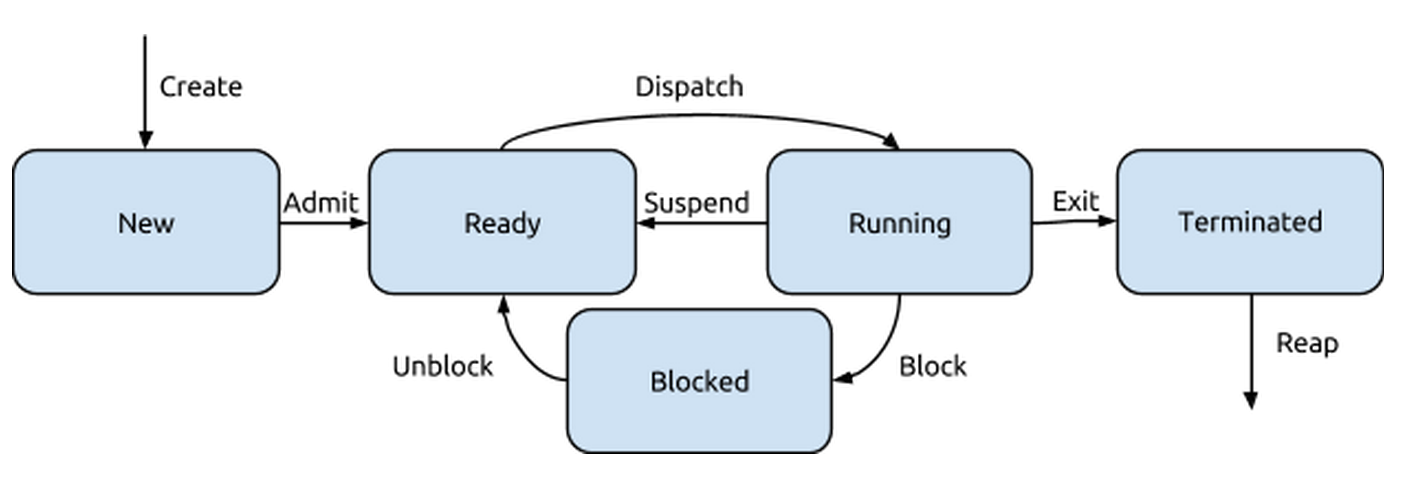
\includegraphics[width=0.85\textwidth]{images/5-state-model.png}\\
State diagram for the five-state model.
\end{center}

There are now eight transitions, most of which are similar to what we have seen before:

\begin{itemize}
	\item \textbf{Create:} The process is created and enters the New state.
	\item \textbf{Admit:} A process in the New state is added to the list of processes ready to start, in the Ready state.
	\item \textbf{Dispatch:} A process that is not currently running begins executing and moves to the Running state.
	\item \textbf{Suspend:} A running program pauses execution, but can still run if allowed, and moves to the Ready state.
	\item \textbf{Exit:} A running program finishes and moves to the Terminated state; its return value is available.
	\item \textbf{Block:} A running program requests a resource, does not get it right away, and cannot proceed.
	\item \textbf{Unblock:} A program, currently blocked, receives the resource it was waiting for; it moves to the Ready state.
	\item \textbf{Reap:} A terminated program's return value is collected by a \texttt{wait} and its resources can be released.
\end{itemize}

There are two additional ``Exit'' transitions that may happen but are not shown. In theory, a process that is in the Ready or Blocked state might transition directly to the Terminated state. This can happen if a process is killed, by the user or by its parent (recall that parent processes can generally kill their children at any time, something the law thankfully does not permit). It may also happen that the system has a policy of killing all the children of a parent process when the parent process dies.

\subsection*{Swapping Processes to Disk}
We can expand on the five state model with something else: the idea that a process might be swapped out to disk rather than in memory. Memory can have multiple processes in it and if the executing process gets blocked, another can be swapped into memory. Unfortunately, however, it is quite possible that the user wants to have more processes running than can currently be accommodated in main memory. The problem is not the PCBs, which are relatively small (a few thousand bytes), but the stack and heap space allocated to the running program can be very large (on the order of gigabytes). 

A first solution that may be attempted is not to allow starting programs when there is not sufficient free space in main memory. This approach falls down on several fronts. First of all, programs do not declare in advance how much memory they will eventually use. Also, a program may not even know how much memory it will need; when you open a text editor to write a program, how can the editor have any idea how long the program is going to be? Even if these were things we could know in advance, users would be most unhappy with this solution. Imagine trying to open a program and being told it can't run because there is insufficient free memory. Memory usage is mostly invisible to the user and incomprehensible, so from his or her perspective the computer would be refusing to launch programs ``randomly''.

Another solution, then: buy more RAM. Memory gets expensive beyond a certain point (otherwise RAM would be 1-2 TB and not 4-16 GB). But there is a saying that ``programs expand to fill the RAM available''\footnote{Employer's version: ``work expands to fill the time available.''}. A computer today might have a thousand times more RAM than it did 20 years ago, but programs today use a thousand times more RAM than the programs of 20 years ago. What we get when we increase the size of memory is not more processes in memory, but larger processes~\cite{osi}.

So, with no other place to put them, we have to put some processes on disk, and this is what we know as swapping. Thus, when the demands for memory exceed the available memory, some of the processes will be moved to disk storage to make room for other processes. This is a notably expensive operation: swapping a process to disk might mean transferring several hundred megabytes of data, or even a few gigabytes, which, from the perspective of the CPU, takes about seven eternities. Then, when that process is going to run again, we need to load it back in to memory, which, again, will take just as much time as it took to flush it out. So this is something to be done only when necessary.

Because we do not want to spend any more time swapping the process in and out of memory than is necessary, (and we need to know if a particular process is in memory or on disk) we need a new state: swapped.  Ideally, we will only swap a process to disk if it is blocked. It cannot run anyway, so if we have to choose a process to put on disk, a blocked one is better than a ready one. A process swapped to disk then enters that sixth state, swapped, which means it is blocked and not in main memory.

There are two scenarios that may have occurred to you that tell us the swapped state on its own is not sufficient. The first is: what if all processes are ready but there is not enough memory space? Or, in other words, what if we need to swap out a process that is ready? The second is: what if the event the blocked process was awaiting has taken place (e.g., the user presses a key) and the process could proceed? How can we tell which processes currently swapped out have had their desired events occur and which have not? We would not like to guess in the second scenario, because swapping a process into memory is time consuming.

The solution to both problem scenarios is to split the swapped state in two: Ready/Swapped (ready to run, and currently not in memory) and Blocked/Swapped (not ready to run, and currently not in memory). That gives us, finally, the seven-state model, a minor variation of the five-state model:

\begin{center}
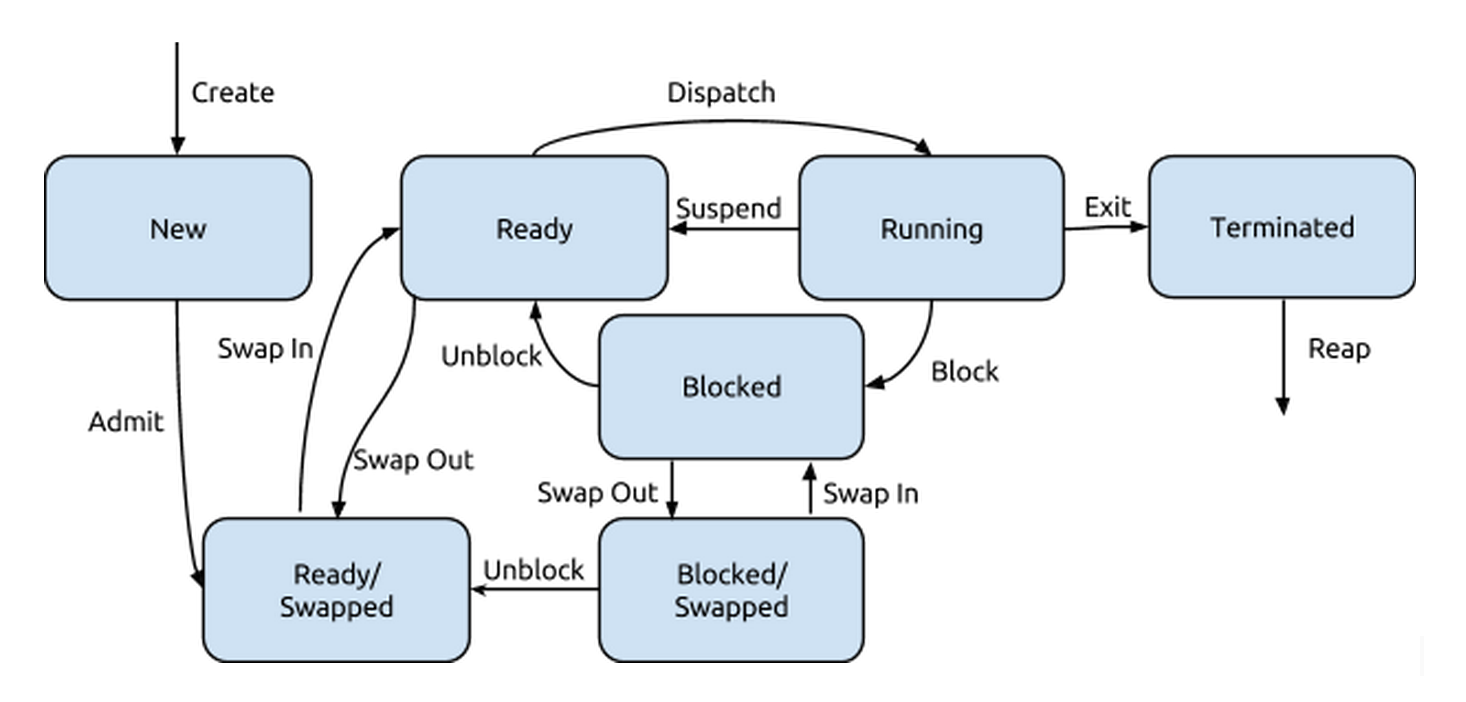
\includegraphics[width=0.85\textwidth]{images/7-state-model.png}\\
State diagram for the seven-state model.
\end{center}

The Admit transition is modified to show that by default the new process does not start in main memory. Two new transitions, Swap In and Swap Out, are added to show a process being loaded into main memory and written out to disk respectively. Finally, there is a second Unblock transition, where a Blocked/Swapped process gets whatever it was waiting for and moves to the Ready/Swapped state, because it can now run (but is still on disk).

As in the five-state model, there are additional ``Exit'' transitions that may happen but are not shown. If a process is killed, for example, regardless of whether it is in memory or on disk, it will move to the Terminated state.

\subsection*{Preview of Scheduling}

Processes, represented by their PCB, are maintained in a data structure; typically a linked list or a queue of some sort. For efficiency reasons, it would not make sense to have all processes in one single linked list that we would have to iterate over. If there are 200 processes and the next ready one is number 137, it's a lot of iterations... So it is logical to take non-ready processes out of this list.

When a process is in some state like ``Blocked'', where does it go? This is a question we will come back to when we discuss scheduling in more detail. But for now, it's convenient for the operating system to keep track of what processes are in which states separately. If a process is waiting for a disk operation, when the disk becomes available, it would be convenient to know quickly what process(es) is(are) waiting for the disk. See the diagram from~\cite{osc}:

\begin{center}
\includegraphics[width=0.55\textwidth]{images/pcbs-in-queues.png}\\
Ready queue and queues on various devices.
\end{center}

A common way of looking at the way processes move around is in a queueing diagram, as in this example from~\cite{osc}, in which each rectangle represents a queue:

\begin{center}
\includegraphics[width=0.55\textwidth]{images/queueing-diagram.png}\\
Queueing diagram for process scheduling.
\end{center}

A process initially goes into the ready queue until it is selected to run, and then it is executing on the CPU. If it makes an I/O request then it will be placed in an I/O queue, for example, until such time as its request is serviced and then it becomes ready again.

How a process is chosen to run next is a major topic, which we will cover later when we get to the discussion about scheduling.

\bibliographystyle{alphaurl}
\bibliography{252}


\end{document}